\documentclass{article}

% if you need to pass options to natbib, use, e.g.: \PassOptionsToPackage{numbers, compress}{natbib} before loading
%     neurips_2020

% ready for submission \usepackage{neurips_2020}

% to compile a preprint version, e.g., for submission to arXiv, add add the [preprint] option:
% \usepackage[preprint]{neurips_2020}

% to compile a camera-ready version, add the [final] option, e.g.: \usepackage[final]{neurips_2020}

\PassOptionsToPackage{numbers, compress}{natbib}

% to avoid loading the natbib package, add option nonatbib:
     \usepackage[preprint]{neurips_2020}

\usepackage[utf8]{inputenc} % allow utf-8 input
\usepackage[T1]{fontenc}    % use 8-bit T1 fonts
\usepackage{hyperref}       % hyperlinks
\usepackage{url}            % simple URL typesetting
\usepackage{booktabs}       % professional-quality tables
\usepackage{amsfonts}       % blackboard math symbols
\usepackage{amsmath}
\usepackage{nicefrac}       % compact symbols for 1/2, etc.
\usepackage{microtype}      % microtypography
\usepackage{listings}
\usepackage{graphicx}
\usepackage{caption}
\usepackage{subcaption}

\title{Auto find mispositioned catheters and lines by deep learning methods}

% The \author macro works with any number of authors. There are two commands used to separate the names and addresses of
% multiple authors: \And and \AND.
%
% Using \And between authors leaves it to LaTeX to determine where to break the lines. Using \AND forces a line break at
% that point. So, if LaTeX puts 3 of 4 authors names on the first line, and the last on the second line, try using \AND
% instead of \And before the third author name.

\author{%
  Fangzhou Ai\\
  Department of Electrical and Computer Engineering\\
  University of California, San Diego\\
  La Jolla, CA 92093 \\
  \texttt{faai@eng.ucsd.edu} \\
  % examples of more authors
   \And Yue Qiao \\
   Department of Electrical and Computer Engineering \\
   University of California, San Diego\\
   La Jolla, CA 92093 \\
   \texttt{yuq021@eng.ucsd.edu}\\
   \And Zunming Zhang \\
   Department of Electrical and Computer Engineering \\
   University of California, San Diego\\
   La Jolla, CA 92093 \\
   \texttt{zuz008@eng.ucsd.edu}\\
}

\begin{document}

\maketitle

\begin{abstract}
     In this paper, we propose a method that can label mispositioned catheters and lines on X-Ray images by using deep
     learning and image classification methods. We used different architectures like Resnet, EfficientNet, and DenseNet
     as the backbone of our solution to classify the line and tube from x-ray photos. We also applied different image
     augmentation methods to enhance our results. We introduced the learning rate scheduling method for fast convergence
     during the training, and we also employed mixed-precision training to accelerate the whole procedure while saving
     the GPU memory. The experiment result shows that the EfficientNet backbone significantly improves the
     classification accuracy compared to ResNet and DenseNet backbone.
\end{abstract}

%--------------------------------------------

\section{Introduction}
In hospitals, mispositioned lines and tubes would cause severe complications in patients. Nowadays, doctors and nurses
frequently use traditional checklists to ensure they follow protocol in managing patients. These steps can be
time-consuming and prone to human error, especially in stressful situations when hospitals are at capacity.

Nasogastric tube mispositioning into the airways has been reported in up to 3\% of cases, with up to 40\% of these cases
demonstrating complications. Airway tube malposition in adult patients intubated outside the operating room is seen in
up to 25\% of cases. The likelihood of complication is directly related to both the experience level and specialty of
the proceduralist. Early recognition of malpositioned tubes is the key to preventing dangerous complications (even
death), even more so now that millions of COVID-19 patients need these tubes and lines.

The gold standard for the confirmation of line and tube positions is chest radiographs in the real world. Once getting
the chest radiographs (X-Ray images), a physician or radiologist must manually check these chest x-rays to verify the
lines and tubes are correctly positioned.  Not only does this leave room for human error, but delays are also common as
radiologists can be busy reporting other scans. Leveraging deep learning, we believe that we could develop algorithms
that may be able to detect mispositioned catheters and lines automatically.  Once alerted, clinicians can reposition or
remove them to avoid life-threatening complications, which will dramatically reduce the human resources involved.

Under the COVID-19 pandemic, almost all the hospitals are at capacity, and more patients require correctly positioned
catheter lines and tubes. If successful, our efforts may help clinicians save lives. Earlier detection of mispositioned
catheters and lines is even more critical as COVID-19 cases continue to surge. Quick feedback on catheter and line
placement could help clinicians better treat these patients. Even beyond COVID-19, detection of line and tube position
will always be required by many ill hospital patients.

The Royal Australian and New Zealand College of Radiologists (RANZCR) is a not-for-profit professional organization for
clinical radiologists and radiation oncologists in Australia, New Zealand, and Singapore. The group is one of many
medical organizations worldwide (including the NHS) that recognizes mispositioned tubes and lines as preventable. To
label mispositioned tubes by deep learning methods, we use the dataset with X-Ray images and handcrafted labels
published by RANZCR on Kaggle\cite{RANZCRCL93:online}.

%--------------------------------------------

\section{Related Work}
Paras Lakhani \cite{lakhani2017deep} evaluated the efficacy of deep convolutional neural networks (DCNNs) in
differentiating subtle, intermediate, and more obvious image differences in radiography. In the paper, three different
datasets were created, which included presence/absence of the endotracheal (ET) tube (n = 300), low/normal position of
the ET tube (n = 300), and chest/abdominal radiographs (n = 120). The datasets were split into training, validation, and
test. Both untrained and pre-trained deep neural networks were employed, including AlexNet and GoogLeNet classifiers,
using the Caffe framework. Data augmentation was performed for the presence/absence and low/normal ET tube datasets.

In\cite{wang2018chestnet}, Hongyu Wang and Yong Xia proposed a model called ChestNet, which consists of two branches: a
classification branch serves as a uniform feature extraction-classification network to free users from troublesome
handcrafted feature extraction, and an attention branch exploits the correlation between class labels and the locations
of patholog-ical abnormalities and allows the model to concentrate adaptively on the patholog-ically abnormal
regions.With this model they achieved SOTA on the Chest X-ray 14 dataset.

In \cite{fridadar2019endotracheal}, Maayan and etc. suggest a method for training the network, first with synthetic data
and then with real X-ray images in a fine-tuning phase, which allows the network to train on thousands of cases without
annotating any data. The proposed method was tested on 477 real chest radiography from a public data set and reached AUC
of 0.99 in classifying the presence vs. absence of the ET tube, along with outputting high quality ET tube segmentation
maps, which could give us more hints on how the training should go on.

%--------------------------------------------
\section{Method}
\subsection{Dataset}
In this paper, we would like to detect the presence and position of catheters and lines on chest x-rays. We use 40,000
images as inputs to train and test our model.

The dataset has been labeled with a set of definitions to ensure consistency with labeling. The normal category includes
lines that were appropriately positioned and did not require repositioning; The borderline category includes lines that
would ideally require some repositioning but would in most cases still function adequately in their current position;
The abnormal category included lines that required immediate repositioning. Since there can be multiple tubes in an
X-Ray image and different tubes have different usages, the dataset labels are further separated into different tube
categories. There are four categories for tubes in the dataset: PAC stands for Pulmonary artery catheter; ETT stands for
endotracheal tube; NGT stands for Nasogastric tube; CVC stands for central venous catheter. The model will output if any
kind of tubes are mispositioned.

\subsection{Architecture}
Convolutional neural network (CNN) is one of the most popular architectures to solve the image classification problem.
ResNet\cite{he2015deep} is one of the most widely used CNN architectures. ResNet features residual learning blocks that
help fight against vanishing gradients problem by introducing skip connections. DenseNet\cite{huang2017densely} connects
each layer to every other layer in a feed-forward fashion. Whereas traditional convolutional networks with L layers have
L connections (one between each layer and its subsequent layer), DenseNet network has L(L+1)/ 2 direct connections. For
each layer, the feature-maps of all preceding layers are used as inputs, and its own feature-maps are used as inputs
into all subsequent layers. DenseNets have several compelling advantages: they alleviate the vanishing-gradient problem,
strengthen feature propagation, encourage feature reuse, and substantially reduce the number of parameters.
EfficientNet\cite{tan2020efficientnet} is a recently introduced convolutional neural network. The authors of
EfficientNet first design a new baseline network using neural architecture search and later scales it up using a new
scaling method that uniformly scales the properties of CNNs using a highly effective compound coefficient. The
EfficientNet series archives state-of-the-art accuracy in the ImageNet dataset as of 2020.

We choose ResNet, DenseNet and EfficientNet as the backbone CNN for our classification model in our experiments. Most of
the published experiments on this dataset use ResNet as their image classification backbone. ResNet series are great
models and are used widely in image classification tasks. However, from the paper and experiments published recently,
EfficientNet performs better than ResNet on ImageNet classification. Therefore, we believe changing the CNN backbone
from ResNet to EfficientNet can improve the accuracy of mispositioned tube detection.

Since there are multiple tubes, we proposed a multi-head image classification network for poorly placed tube detection.
In our model, we have four different heads. Each of them receives the same flattened CNN features as input and uses a
single linear layer for classification output. We use different loss functions for different heads. For ETT and SGC
heads, we applied a standard Softmax layer and cross-entropy loss on them. For NGT and CVC heads, we applied a Sigmoid
layer and Binary cross-entropy loss on them. We use Binary cross entropy loss on NGT and CVC heads because there could
be more than one NGT or CVC tubes in one X-Ray image. Therefore, the result can be both in the Normal category and
Abnormal Category. The traditional Softmax layer does not fit this situation, so we use a sigmoid layer and Binary
cross-entropy loss.

One of the critical properties of CNN is that the shallow layers in CNN learn general features. In contrast, the deep
layers in CNN learn specific features. Using this property, we also propose a new kind of header with an extra CNN layer
and a linear layer.  The CNN layer is the same as the last layer of the CNN backbone. In training, the heads receive
features from the second to last layer of the CNN backbone and extract features using the last CNN layer with its own
weights. We believe this kind of head can perform better because it can only learn the specific feature it wants.

\subsection{Image augmentation}
Image augmentation is a common technique used in image classification tasks. To archive higher accuracy, deep learning
methods require many samples. However, the samples available for training are usually limited. We can use image
augmentation to create new training samples artificially by rotation, crop, and flip the images to solve the problem. In
our settings, we first scale the images by a random multiplier with a range of 0.08 to 1.0; then, we crop the image to
256x256. The cropping process reduces the GPU memory usage in training and ensures that image processing is fast since
the original images are large. After random rotation and random flip are applied to the image, we normalize the image to
the mean and the standard deviation from the ImageNet dataset. The normalizing process solves the imbalance samples
problem and ensures smooth training as we apply weights pre-trained on ImageNet to our CNN backbones.

\subsection{Learning rate scheduling}
To archive the best accuracy, we dynamically reduce the learning rate during training. We use a method called reducing
learning rate on plateau. As the name tells, half of the learning rate will be reduced if the validation set's overall
accuracy has stopped increasing for 10 epochs. We use this method to accelerate the initial learning by using a slightly
larger learning rate and fine-tuning the model automatically by reducing the learning rate.

\subsection{Mixed precision training}
As recent CNN models become deeper and deeper, GPU memory requirement increases, and the training speed decreases. We
use a new training method called mixed-precision training to accelerate the training speed and reduce GPU memory usage.
During training, all convolution and matrix multiplication will be performed under float 16 precision, significantly
reducing GPU memory usage by half and increasing training speed. When calculating loss, the precision is scaled back to
float 32 to prevent underflow or overflow for loss calculation.

\section{Experiments}
We split the official dataset into the training set and validation set, and use a fixed random seed to ensure the result
is reproducible. $80\%$ percent of data becomes training set, $10\%$ of data becomes validation set, and $10\%$ of
data becomes test set. During the training, we use SGD as the optimizer, set the batch size to $32$, initial
learning rate to $0.001$ and momentum to $0.9$. We use PyTorch as our training framework and use Tensorboard to monitor
and record our training results.

\subsection{Metrics}

Instead of looking at the results' accuracy, we use area under ROC curve (AUC) as our metrics. A ROC curve (receiver
operating characteristic curve) shows the true positive rate and false positive rate of a binary classification model at
all classification thresholds. AUC is the area under the ROC curve, which is classification threshold invariant. Since
people can set a threshold based on their needs (more false positive or false negative), the AUC metric can better
reflect a binary classification model's overall performance.

\subsection{Results}

\paragraph{Compare between different CNN models}
The overall Loss and AUC is shown in \autoref{fig:cnn_val_overall}. All of the models use CNN + Linear head.

\begin{figure}[h]
     \centering
     \begin{subfigure}[b]{0.49\textwidth}
          \centering
          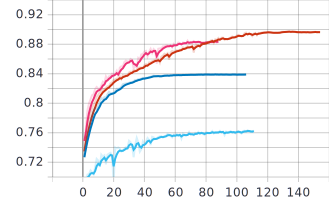
\includegraphics[width=\textwidth]{cnn_val_auc.png}
          \caption{Overall AUC}
          \label{fig:cnn_val_auc}
     \end{subfigure}
     \hfill
     \begin{subfigure}[b]{0.49\textwidth}
          \centering
          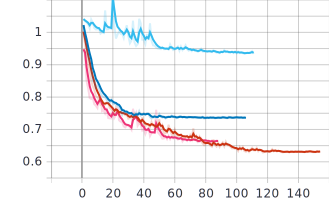
\includegraphics[width=\textwidth]{cnn_val_loss.png}
          \caption{Overall loss}
          \label{fig:cnn_val_loss}
     \end{subfigure}
     \caption{Overall Loss and AUC for different CNN backbone. Pink line: Model with ResNet50 backbone. \
          Red line: Model with EfficientNet-b5 backbone.Blue line: Model with EfficientNet-b4 backbone. \
          Aqua line: Model with DenseNet201 backbone.}
     \label{fig:cnn_val_overall}
\end{figure}

The validation AUC for different categories is shown in \autoref{fig:cnn_categories_val_auc}.

\begin{figure}[h]
     \centering
     \begin{subfigure}[b]{0.49\textwidth}
          \centering
          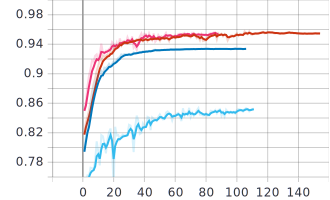
\includegraphics[width=\textwidth]{cnn_val_auc_ett.png}
          \caption{ETT AUC}
          \label{fig:cnn_val_auc_ett}
     \end{subfigure}
     \hfill
     \begin{subfigure}[b]{0.49\textwidth}
          \centering
          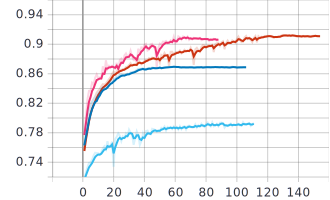
\includegraphics[width=\textwidth]{cnn_val_auc_ngt.png}
          \caption{NGT AUC}
          \label{fig:cnn_val_auc_ngt}
     \end{subfigure}
     \hfill
     \begin{subfigure}[b]{0.49\textwidth}
          \centering
          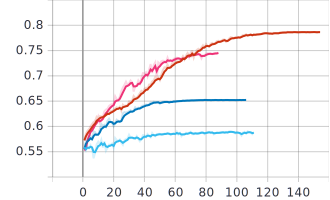
\includegraphics[width=\textwidth]{cnn_val_auc_cvc.png}
          \caption{CVC AUC}
          \label{fig:cnn_val_auc_cvc}
     \end{subfigure}
     \hfill
     \begin{subfigure}[b]{0.49\textwidth}
          \centering
          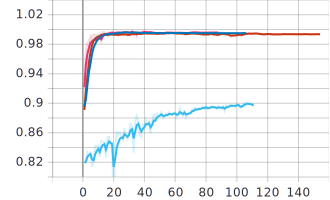
\includegraphics[width=\textwidth]{cnn_val_auc_sgc.png}
          \caption{SGC AUC}
          \label{fig:cnn_val_auc_sgc}
     \end{subfigure}
     \caption{Validation AUC for different tube categories. Pink line: Model with ResNet50 backbone. \
          Red line: Model with EfficientNet-b5 backbone.Blue line: Model with EfficientNet-b4 backbone. \
          Aqua line: Model with DenseNet201 backbone.}
     \label{fig:cnn_categories_val_auc}
\end{figure}

The test AUC for different CNN models is shown in \autoref{table:cnn_auc}.

\begin{table}[h]
     \caption{AUC on test set for different CNN models}
     \label{table:cnn_auc}
     \centering
     \begin{tabular}{@{}ll@{}}
          \toprule
          Model           & Testset AUC \\
          \midrule
          Resnet-50       & 0.8835      \\
          EfficientNet-b4 & 0.8389      \\
          EfficientNet-b5 & 0.8973      \\
          DenseNet201     & 0.7622      \\
          \bottomrule
     \end{tabular}
\end{table}

\paragraph{Compare between different heads}
The overall AUC for differrnt heads shown in \autoref{fig:cnn_val_overall}.

\begin{figure}[h]
     \centering
     \begin{subfigure}[b]{0.49\textwidth}
          \centering
          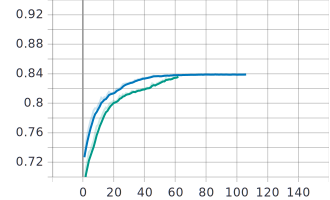
\includegraphics[width=\textwidth]{head_efficientnet_val_auc.png}
          \caption{EfficientNet-b4 AUC. Blue line: CNN + Linear layer. Green line: Linear layer.}
          \label{fig:head_efficientnet_val_auc}
     \end{subfigure}
     \hfill
     \begin{subfigure}[b]{0.49\textwidth}
          \centering
          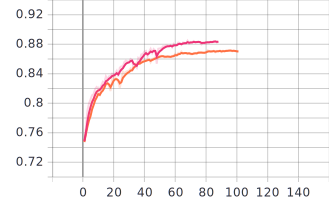
\includegraphics[width=\textwidth]{head_resnet_val_auc.png}
          \caption{ResNet-50 AUC. Pink line: CNN + Linear layer. Orange line: Linear layer.}
          \label{fig:head_resnet_val_auc}
     \end{subfigure}
     \caption{Overall AUC for different heads.}
     \label{fig:head_val_overall}
\end{figure}

The test AUC for different CNN models is shown in \autoref{table:head_auc}.

\begin{table}[h]
     \caption{AUC on test set for different head}
     \label{table:head_auc}
     \centering
     \begin{tabular}{@{}ll@{}}
          \toprule
          Head-Model                & Testset AUC \\
          \midrule
          Linear-Resnet-50          & 0.8698      \\
          CNNLinear-Resnet-50       & 0.8835      \\
          Linear-EfficientNet-b4    & 0.8389      \\
          CNNLinear-EfficientNet-b4 & 0.8377      \\
          \bottomrule
     \end{tabular}
\end{table}

\section{Discussion}

From \autoref{fig:cnn_val_overall}, we can see that EfficientNet-b5 has the highest AUC. It is expected since it is the
largest model among all of the four models. The ResNet-50 performs better than we expected. It has almost the same
performance as EfficientNet-b5 on ETT, and outperforms EfficientNet-b4 on all categories. Recent work has shown that
convolutional networks can be more accurate and efficient to train if there are more short connections in and between
layers. DenseNets take this into consideration and develop the architecture. But from this experiment, we could see that
the AUC for DenseNet is the lowest. One possible reason is that these skip connecctions in DenseNet destory the layer
structure and the individual CNN layers in the heads are actually affecting each other.

Comparing AUC for different heads using data in \autoref{fig:head_val_overall}, we can see that CNN + Linear layer head
works better for both models. The result is consistent with what we expected before: shallow CNN layers learn general
features; deep CNN layers learn specific features. With one layer more flexibility of learning, the whole model will
work better.


\section{Individual contributions to the project}

\paragraph{Fangzhou Ai}
Fine tuning.

\paragraph{Yue Qiao}
ResNet and EfficientNet model. Multi-Head design.

\paragraph{Zunming Zhang}
DenseNet model.

%--------------------------------------------

\bibliographystyle{plainnat}
\bibliography{bibfile}

\end{document}